    \section{Segmentierung}

Dieses ist die Zerlegung eines Bildes in verschiedene Objekt.\\
Eine einfache Methode hierfür ist das \textbf{Histogramm thresholding}\index{Histogramm thresholding}:
\begin{center}
  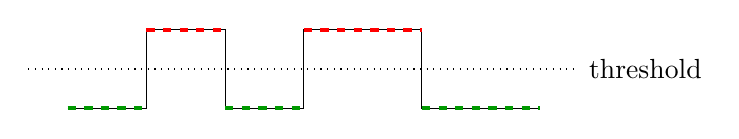
\begin{tikzpicture}
    \draw (1,0) -- (2,0) -- (2,1) -- (3,1) -- (3,0) -- (4,0) -- (4,1) -- (5.5,1) -- (5.5,0) -- (7,0);
    \draw[dotted] (0.5,0.5) -- (7.5,0.5) node[right] {threshold};
    \draw[line width=0.5mm,red,dashed] (2,1) -- (3,1);
    \draw[line width=0.5mm,red,dashed] (4,1) -- (5.5,1);
    \draw[line width=0.5mm,green!60!black,dashed] (1,0) -- (2,0);
    \draw[line width=0.5mm,green!60!black,dashed] (3,0) -- (4,0);
    \draw[line width=0.5mm,green!60!black,dashed] (5.5,0) -- (7,0);
  \end{tikzpicture}
\end{center}
So kann ein Bild in mehrere Objekte zerlegt werden.\\
Hierbei können jedoch diverse Probleme auftreten, die vor der Zerlegung durch preprocessing behoben werden sollten. Einige der preprocessing Methoden sind:
\begin{enumerate}
  \item[-] Entrauschen $\nearrow$ 5.7
  \item[-] Farbraum optimal ausnutzen $\nearrow$ 3.2
  \item[-] \textbf{Beleuchtungsausgleich}\index{Beleuchtungsausgleich}
\end{enumerate}
Dieser Beleuchtungsausgleich wurde noch nicht vorher besprochen, das Problem:

\begin{center}
  \begin{tikzpicture}
    \draw (0,0) -- ++(20:1) -- ++(0,1) -- ++(20:1) -- ++(0,-1) -- ++(20:1) -- ++(0,1) -- ++(20:1.5) -- ++(0,-1) -- ++(20:1.5);
    \draw[dotted] (-0.5,1.5) -- (6,1.5) node[right] {threshold??};
  \end{tikzpicture}
\end{center}

Anstatt eines \quo{geraden} Bildes ist das Bild, etwa durch Beleuchtung, \quo{gekippt} und der Ansatz mittels Histogramthresholding würde nicht das gewünschte Ergebnis erzielen.\\

In 2D könnte dies so aus sehen.

\begin{center}
  \begin{tikzpicture}
    \draw[white] (0,0) rectangle node[draw,black] {
\includegraphics[scale = 0.2]{Bild3plusgrad.png}} (3,3);
    \draw (1.5,3) node[above] {\LARGE $f$};
    \draw (1.5,0) node[below] {gegeben};
    \draw (3.5,1.5) node[] {\LARGE $=$};
    \draw[white] (4,0) rectangle node[draw,black] {
\includegraphics[scale = 0.2]{Bild3.png}} (7,3);
    \draw (5.5,3) node[above] {\LARGE $u$};
    \draw (5.5,0) node[below] {erwünscht};
    \draw (7.5,1.5) node[] {\LARGE $+$};
    \draw[white] (8,0) rectangle node[draw,black] {
\includegraphics[scale = 0.2]{Bild3grad.png}} (11,3);
    \draw (9.5,3) node[above] {\LARGE $v$};
    \draw (9.5,0) node[below] {gesucht};
    \draw (11.75,1.5) node[] {\LARGE $\Longleftrightarrow$};
    \draw[white] (12.5,0) rectangle node[draw,black] {
\includegraphics[scale = 0.2]{Bild3thresh.png}} (15.5,3);
    \draw (14,3) node[above] {};
    \draw (14,0) node[below] {Ergebnis durch thresholding};
  \end{tikzpicture}
\end{center}

Rechts ist das Bild, das durch das Beschriebene Histogramm thresholding dargestellt wurde zu sehen. Methoden um durch preprocessing den gesuchten Gradienten zu entfernen werden im folgenden beschrieben.

\subsection{Beleuchtungsausgleich}

\begin{enumerate}[label = ]
    \item Geg.: inhomogen ausgeleuchtetes Bild $f$.
    \item Ges.: Zerlegung $f = u + v$, wobei
        \begin{enumerate}[label = ]
            \item $u$ erwünschter Anteil,
            \item $v$ Inhomogenität .
        \end{enumerate}
\end{enumerate}
Gilt $f = u \cdot v$ (multiplikative Verknüpfung) so erhält man den obigen Fall durch Betrachtung des Logarithmus $\log(f)$.

\begin{enumerate}
  \item[Einfachster Fall:] $v$ konstant. In diesem Fall kann man etwa eine \quo{Leeraufnahme} machen, $v=f$ setzen und dieses $v$ in allen folgenden Aufnahmen subtrahieren.
  \item[Normalfall:] $v$ ändert sich bei Jeder Aufnahme. Hierbei gibt es mehrere Ansätze:
\end{enumerate}

\begin{enumerate}[label = \alph*)]
    \item \textbf{Lineare Regression}\index{Lineare Regression}: \\
  \begin{minipage}[c]{0.6\linewidth}
  \item[] Wir unterstellen, dass der Verlauf \textbf{affin-linear}\index{affin-linear} ist, d.h.:
          \[v(x,y) = a x + b y + c\]
          Diese Parameter $a$, $b$, $c$ gilt es nun so zu schätzen.
    \end{minipage}
    \hfill
    \begin{minipage}[c]{0.35\linewidth}
              \begin{center}
        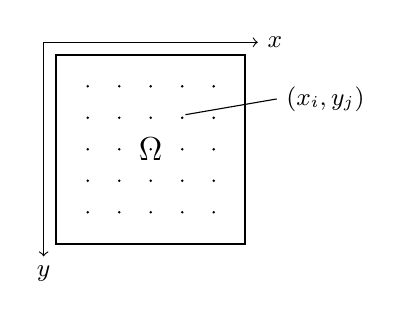
\begin{tikzpicture}[scale=0.8]
          \draw[thick] (0,0) rectangle node[] {\large $\Omega$} (3,3);
          \draw[->] (-0.2,3.2) -- (3.2,3.2) node[right] {\small $x$};
          \draw[->] (-0.2,3.2) -- (-0.2,-0.2) node[below] {\small $y$};
          \foreach \x in {1,...,5}
            \foreach \y in {1,...,5}{
              \draw (\x / 2,\y / 2) node[circle,fill=black,inner sep=0pt] {};
          }
          \draw (2.05,2.05) -- (3.5,2.3) node[right] {\small $(x_i,y_j)$};
        \end{tikzpicture}
      \end{center}
    \end{minipage}
    Dazu soll gelten
    \[\forall (x,y) \in \Omega \colon\quad ax+by+c \approx f(x,y).\]
    Um dies zu erfüllen wird eine Stichprobe von endlich vielen Punkten $(x_i,y_i)$ aus $\Omega$ gewählt und durch diese ein Gleichungssystem gebildet:
    \begin{gather*}
    ax_1+by_1+c \approx f(x_1,y_1)\\
    \vdots \\
    ax_n+by_n+c \approx f(x_n,y_n)
    \end{gather*}
    In Matrix Form ergibt sich:
    \[\underbrace{\mat{x_1 & y_1 & 1 \\ \vdots & \vdots & \vdots \\ \vdots & \vdots & \vdots \\ \vdots & \vdots & \vdots \\ x_n & y_n & 1}}_{A} \underbrace{\mat{a \\ b \\ c}}_{w} \approx \underbrace{\mat{f(x_1,y_1) \\ \vdots \\ \vdots \\ \vdots \\ f(x_n,y_n)}}_{z}\]
    Wir erhalten also ein lineares Ausgleichsproblem (überbestimmtes Gleichungssystem).
    Die optimale Lösung dieses Problems kann über die \textbf{Normalengleichung}\index{Normalengleichung} berechnet werden:
    \[A^T A w = A^T z.\]
    Daraus erhält man $w$, somit auch $a$, $b$, $c$ und schlussendlich $v \Rightarrow u = f-v$.\\
    Eventuell wird durch die Subtraktion bei $u$ der Farbraum verlassen.
    Anschließend wird daher noch ein Histogramm stretching durchgeführt, um das finale Bild zu erhalten.

\item \textbf{Polynomiale Regression}\index{Polynomiale Regression}:
    Ähnlich zur linearen Regression wird hierbei keine affin-lineare Funktion, sondern ein Polynom genutzt. Für ein Polynom zweiten Grades kann etwa die Funktion
    \[v(x,y) = ax^2 by^2 cxy+ dx +ey +f\]
    gewählt werden. Wieder entsteht ein Gleichungssystem:
    \[
    \underbrace{\mat{x_1^2 & y_1^2 & x_1y_1 & x_1 & y_1 & 1 \\ 
                    \vdots & \vdots & \vdots & \vdots & \vdots & \vdots \\ 
                    \vdots & \vdots & \vdots & \vdots & \vdots & \vdots \\ 
                    \vdots & \vdots & \vdots & \vdots & \vdots & \vdots \\ 
                    x_n^2 & y_n^2 & x_ny_n & x_n & y_n & 1}}_{A} 
        \underbrace{\vphantom{\mat{f(x_1,y_1 \\ \vdots \\ \vdots \\ \vdots \\ f(x_n,y_n)}}
    \mat{a \\ b \\ c \\ d \\e \\ f}}_{w} 
\approx \underbrace{\mat{f(x_1,y_1) \\ \vdots \\ \vdots \\ \vdots \\ f(x_n,y_n)}}_{z}\]

  \item \textbf{Trigonometrisches Polynom}\index{Trigonometrisches Polynom}:
      Hierbei wird $v$ in den niedrigfrequenten Anteilen von $f$ (großflächiger Verlauf, keine Details) gesucht.

  \begin{center}
    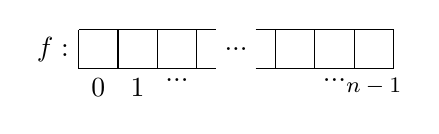
\begin{tikzpicture}
      \draw (0,0.25) node[left] {$f:$};
      \draw[step = 0.5] (0,0) grid (1.75,0.5);
      \draw (2,0.25) node[] {$...$};
      \draw[step = 0.5] (2.25,0) grid (4,0.5);
      \draw (0.25,0) node[below] {$0$};
      \draw (0.75,0) node[below] {$1$};
      \draw (1.25,0) node[below] {$...$};
      \draw (3.25,0) node[below] {$...$};
      \draw (3.75,0) node[below] {\footnotesize $n-1$};
    \end{tikzpicture}
  \end{center}

  Es ergibt sich $\hat f$:

  \[\hat f_k = \sum_{m=0}^{n-1} f_k \bigl(\underbrace{e^{- i 2 \pi \frac{k}{n}}}_{w_k}\bigr)^m \quad , \ k= 0,1,...,n-1\]

  Mittels der FFT (Fast Fourier Transformation) ergibt sich $\hat f$ zu:

  \begin{center}
    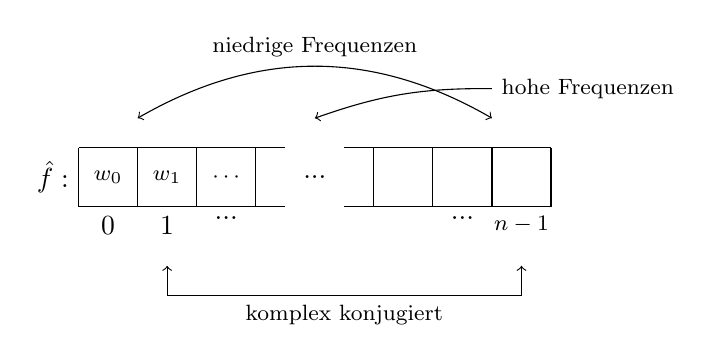
\begin{tikzpicture}[scale=1.5]
      \draw (0,0.25) node[left] {$\hat f:$};
      \draw[step = 0.5] (0,0) grid (1.75,0.5);
      \draw (2,0.25) node[] {$...$};
      \draw[step = 0.5] (2.25,0) grid (4,0.5);
      \draw (0.25,0) node[below] {$0$};
      \draw (0.75,0) node[below] {$1$};
      \draw (0.25,0.25) node[] {\footnotesize $w_0$};
      \draw (0.75,0.25) node[] {\footnotesize$w_1$};
      \draw (1.25,0) node[below] {$...$};
      \draw (3.25,0) node[below] {$...$};
      \draw (1.25,0.25) node[] {\footnotesize$\cdots$};
      \draw (3.75,0) node[below] {\footnotesize $n-1$};
      \draw[<->] (0.75,-0.5) -- (0.75,-0.75) -- node[below] {\footnotesize komplex konjugiert} (3.75,-0.75) -- (3.75,-0.5);
      \draw[<->] (0.5, 0.75) to[bend left] node [above] {\footnotesize niedrige Frequenzen} (3.5,0.75);
      \draw[<-] (2,0.75) to[bend left=10] (3.5,1) node[right] {\footnotesize hohe Frequenzen};
    \end{tikzpicture}
  \end{center}
  Durch entfernen dieser niedrigen Frequenzen ergibt sich $u$.
Ähnliches funktioniert auch in 2D:

    \begin{center}
    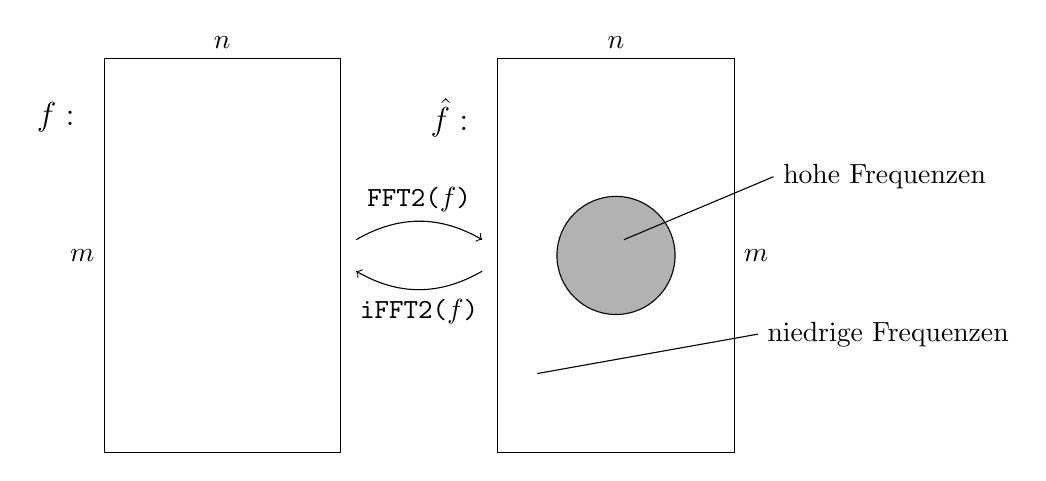
\begin{tikzpicture}[scale=1]
      \draw (0,0) rectangle (3,5);
      \draw (1.5,5) node[above] {$n$};
      \draw (0,2.5) node[left] {$m$};
      \draw (-0.25,4.25) node[left] {\large $f:$};
      \draw[->] (3.2,2.7) to[bend left] node[above] {\tt{FFT2($f$)}} (4.8,2.7);
      \draw[<-] (3.2,2.3) to[bend right] node[below] {\tt{iFFT2($f$)}} (4.8,2.3);
      \draw (5,0) rectangle (8,5);
      \draw (6.5,5) node[above] {$n$};
      \draw (8,2.5) node[right] {$m$};
      \draw (4.75,4.25) node[left] {\large $\hat f:$};
      \draw[fill = black!30] (6.5,2.5) circle (0.75);
      \draw (6.6,2.7) -- (8.5,3.5) node[right] {hohe Frequenzen};
      \draw (5.5,1) -- (8.3,1.5) node[right] {niedrige Frequenzen};
    \end{tikzpicture}
  \end{center}
\end{enumerate}

\subsection{Thresholding als Variationsproblem}

\begin{enumerate}
\item[geg:] Bild $u: \Omega \to F=[0,1]$ und Schwellenwert $t \in (0,1)$.
\item[$\Rightarrow$:]   $\begin{array}{lr}
                            \Omega_0 = \{x \in \Omega : u(x) \leq t \} \to \text{schwarz}  \\
                            \Omega_1 = \{x \in \Omega : u(x) > t \} \to \text{weiß}
                        \end{array} \bigg \}$ soll in ein Variationsproblem umformuliert werden.
\end{enumerate}

Setze dazu:
\begin{equation}\label{eq.9.1}
J(v) \coloneqq -\int_\Omega (u(x) -t) \C v(x) \d x \to \min
\end{equation}

mit $v \in U \coloneqq  \bigl \{ v \in \Omega \to \{ 0,1\} \text{ \ (oder $[0,1]$)} \bigr\}$, dies ist jedoch kein Vektorraum.

Die Lösung dieses Problems ist offenbar
\[v(x) = \chi_{\Omega_1}(x) =  \begin{cases}
0, & x \in \Omega_0 \\
1, & x \in \Omega_1
\end{cases} \]
illustiert hier:


\begin{center}
    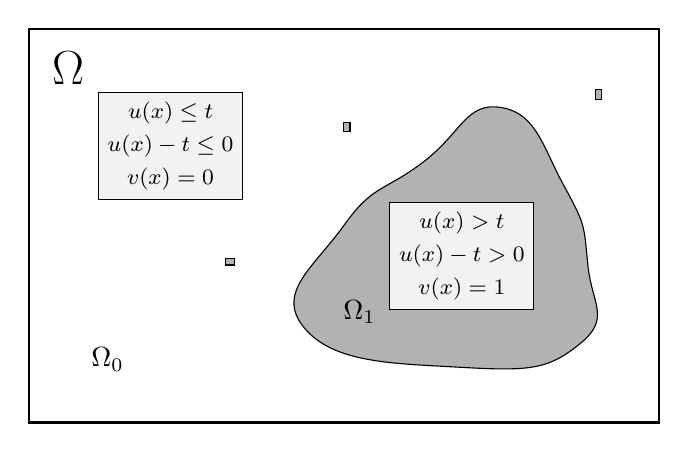
\begin{tikzpicture}
        \draw[thick] (0,0) rectangle (8,5);
        \draw[fill, black!30, draw = black] plot[smooth cycle,tension=0.9] coordinates {(7,1) (7.1,2) (6.8,3) (6,4) (5,3.3) (4,2.5) (3.5,1.2) (5.5,0.7) };
        \draw (0.5,4.5) node[] {\LARGE $\Omega$};
        \draw[white] (0.3, 4.2) -- node[black,below,sloped,style={align=center},draw,fill=black!5] {\footnotesize $u(x) \leq t$ \\ \footnotesize $u(x) -t \leq 0$ \\ \footnotesize $v(x) = 0$} ++(0:3);
        \draw (1,0.8) node[] {$\Omega_0$};
        \draw[] (5.5, 2.8)  node[black,below,sloped,style={align=center},draw,fill=black!5] {\footnotesize $u(x) > t$ \\ \footnotesize $u(x) -t > 0$ \\ \footnotesize $v(x) = 1$};
        \draw (4.2,1.4) node[] {$\Omega_1$};
        \draw[fill, black!30, draw = black] (2.5,2) rectangle ++(0.11,0.08);
        \draw[fill, black!30, draw = black] (4,3.7) rectangle ++(0.08,0.11);
        \draw[fill, black!30, draw = black] (7.2,4.1) rectangle ++(0.07,0.13);
    \end{tikzpicture}
\end{center}

Diese Herangehensweise ist jedoch kompliziert, um sie zu begründen betrachten wir die Flecken die neben der großen Masse in der obigen Illustration zu sehen sind und etwa durch Rauschen entstanden seien könnten. Durch Verallgemeinerung des in \ref{eq.9.1} gegebenen Funktionals können wir die Zerlegung von $\Omega$ in $\Omega_0$ und $\Omega_1$ weniger anfällig gegenüber Rauschen und sonstigen kleinen Strukturen machen.

Dazu sei
\begin{equation}\label{eq.9.2}
\TV(v) \coloneqq \int_\Omega \abs{\nabla v(x)} \d x
\end{equation}

die sogennate \textbf{Totalvariation}\index{Totalvariation} einer Funktion $v$ auf $\Omega$.

Illustration in 1D:
\begin{center}
    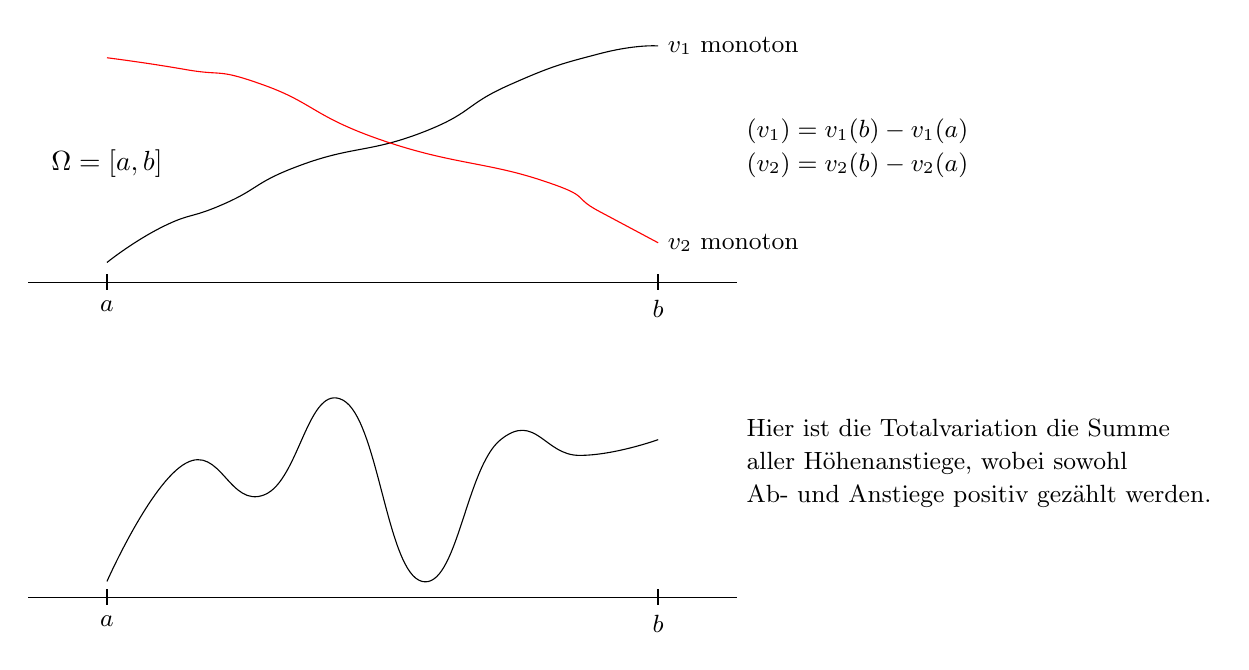
\begin{tikzpicture}
        \draw (0,0) -- (9,0);
        \draw (1,1.5) node[] {$\Omega = [a,b]$};
        \draw plot[smooth,tension=0.9] coordinates {(1,0.25) (1.7,0.7) (2.5,1) (3.5,1.5) (5,1.9) (6.1,2.5) (7.25,2.9) (8,3)} node[right] {\small $v_1$ monoton};
        \draw[red] plot[smooth,tension=0.9] coordinates {(1,2.85) (2,2.7) (3,2.5) (4.5,1.8)  (6.5, 1.3) (7.25,0.9) (8,0.5)} node[black,right] {\small $v_2$ monoton};
        \draw[thick] (1,0.1) -- (1,-0.1) node[below] {\small $a$};
        \draw[thick] (8,0.1) -- (8,-0.1) node[below] {\small $b$};
        \draw (9,1.7) node[style={align=left},right] {\small $\TV(v_1) = v_1(b) -v_1(a)$ \\ \small $\TV(v_2) = \abs{v_2(b) - v_2(a)}$};
        \draw (0,-4) -- (9,-4);
        \draw plot[smooth,tension=0.8] coordinates {(1,-3.8) (2,-2.3) (3, -2.7) (4,-1.5) (5,-3.8) (6,-2) (7,-2.2) (8,-2)};
        \draw[thick] (1,-3.9) -- (1,-4.1) node[below] {\small $a$};
        \draw[thick] (8,-3.9) -- (8,-4.1) node[below] {\small $b$};
        \draw (9,-2.3) node[style={align=left},right] {\small Hier ist die Totalvariation die Summe \\ \small aller Höhenanstiege, wobei sowohl \\
        \small Ab- und Anstiege positiv gezählt werden.};
    \end{tikzpicture}
\end{center}

In Abschnitt \ref{11.2} werden wir weiterhin sehen, dass die Totalvariation sich auch auf nicht stetigen Funktionen etwa $\chi_{(0,\infty)}$ berechnen lässt, obwohl für diese der Gradient nicht definiert ist. Für die eben genannte Funktion etwa beträgt die Totalvariation $1$.

Nun in 2D:
\begin{center}
    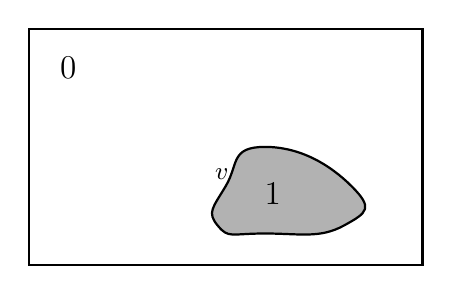
\begin{tikzpicture}
        \draw[thick] (0,0) rectangle (5,3);
        \draw[fill, black!30, draw = black, thick] plot[smooth cycle,tension=1] coordinates {(4,0.5) (4.1,1) (3,1.5) (2.5,1) (2.4,0.5) (3,0.4)};
        \draw (0.5,2.5) node[] {\large $0$};
        \draw (3.1,0.9) node[] {\large $1$};
        \draw (2.45,1.15) node[] {\small $v$};
    \end{tikzpicture}
\end{center}
$\TV(v)$ ist hier die Länge der Kante die $\Omega_1$ von $\Omega_0$ trennt.
Die Idee ist nun $TV(v)$ als Strafterm zu \ref{eq.9.1} hinzu zu addieren,
\begin{equation}\label{eq.9.3}
\widetilde J(v) \coloneqq  \underbrace{-\int_\Omega (u(x)-t) \C v(x) \d x}_{J(x)} + \lambda \C TV(v) \to \min
\end{equation}
wobei $v \in U$ ist.

Der Effekt dieser Herangehensweise wird nun illustriert:
\begin{center}
    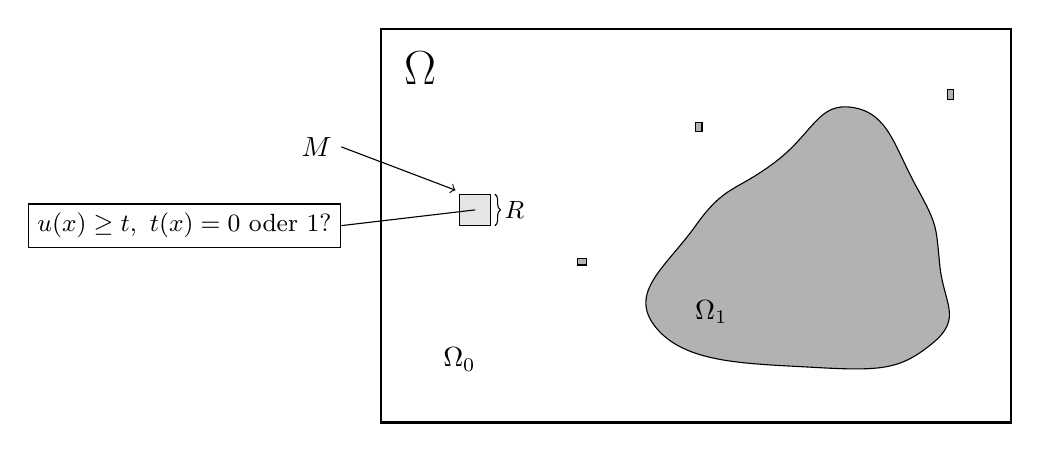
\begin{tikzpicture}
        \draw[thick] (0,0) rectangle (8,5);
        \draw[fill, black!30, draw = black] plot[smooth cycle,tension=0.9] coordinates {(7,1) (7.1,2) (6.8,3) (6,4) (5,3.3) (4,2.5) (3.5,1.2) (5.5,0.7) };
        \draw (0.5,4.5) node[] {\LARGE $\Omega$};
        \draw (1,0.8) node[] {$\Omega_0$};
        \draw (4.2,1.4) node[] {$\Omega_1$};
        \draw[fill, black!30, draw = black] (2.5,2) rectangle ++(0.11,0.08);
        \draw[fill, black!30, draw = black] (4,3.7) rectangle ++(0.08,0.11);
        \draw[fill, black!30, draw = black] (7.2,4.1) rectangle ++(0.07,0.13);
        \draw[fill, black!10, draw = black] (1,2.5) rectangle ++(0.4,0.4);
        \draw[->] (-0.5,3.5) node[left] {$M$} -- (0.95,2.95);
        \draw[] (-0.5,2.5) node[left,draw] {\small $u(x) \geq t, \ t(x)=0$ oder $1$?} -- (1.2,2.7);
        \draw[decorate,decoration={brace,amplitude=2pt}] (1.45,2.9) -- node[right] {\small $R$} (1.45,2.5);
    \end{tikzpicture}
\end{center}

$\begin{array}{cccccccc}
\text{Falls:} & v|_M = 0:&a & +& \lambda \C b \\
\text{Falls:} & v|_M = 1:&a-dR^2 & + &\lambda \C (b+4R)
\end{array} \bigg \}$ Also $M \to 0 \iff 4 \lambda - dR < 0 \iff R > \frac{4 \lambda}{d}$ %??

Das heißt das kleine Segment $M$ wird durch \ref{eq.9.3} \quo{erkannt} falls seine Kantenlänge $R>\frac{4 \lambda}{d}$ ist. Somit können die Abmessung der kleinsten zu segmentierenden Strukturen über $\lambda$ gesteuert werden.

\subsection{Segmentierung nach Mumford und Shah}

\begin{minipage}{.65\textwidth}
    \begin{enumerate}
        \item[Wieder:] Variationsrechnung
        \item[Diesmal:] Ohne Vorkenntnis des thresholds
        \item[Idee:] Bild zerlegen in \quo{glatte} Teile getrennt durch Sprünge an deren Rändern.
        \item[] \
        \item[geg.:] Bild $u$
        \item[ges.:] Stückweise glattes Bild $v$ mit Randkurve $\Gamma$
    \end{enumerate}
    \begin{enumerate}
        \item[1. Wunsch:] $u \approx v$ auf ganz $\Omega$
        \item[2. Wunsch:] $\nabla v$ klein auf $\Omega \backslash \Gamma$
    \end{enumerate}
\end{minipage}%
\begin{minipage}{0.3\textwidth}
\begin{center}
    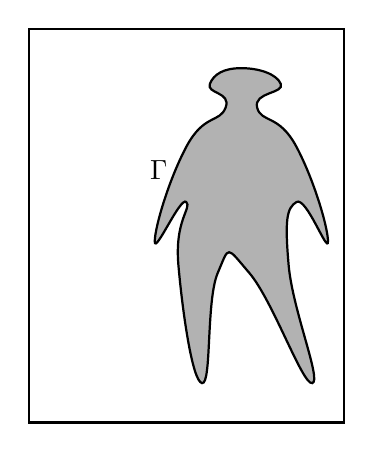
\begin{tikzpicture}
        \draw[thick] (0,0) rectangle (4,5);
        \draw[fill, black!30, draw = black,thick] plot[smooth cycle,tension=0.9] coordinates {(3.6,0.5) (3.3,2) (3.4,2.8) (3.8,2.3) (3.4,3.5) (2.9,4) (3.2,4.3) (2.7,4.5) (2.3,4.3) (2.5,4)  (2,3.5) (1.6,2.3) (2,2.8) (1.9,2) (2.2,0.5) (2.4,1.9) (2.8,1.9)};
        \draw (1.65,3.2) node[] {$\Gamma$};
    \end{tikzpicture}%%(2.7,4)
\end{center}
\end{minipage}

\[\Rightarrow J(v,\Gamma)  \coloneqq  \underbrace{\norm{u-v}_{2,\Omega}^2}_{1. \text{ Wunsch}}  + \lambda \underbrace{\norm{\nabla v}_{2,\Omega \backslash \Gamma}^2}_{2. \text{ Wunsch}} \to \min \]

Wie im letzten Abschnitt \ref{eq.9.2} soll nun noch die Segmentierung sehr kleiner Strukturen vermieden werden, indem man zu $J$ einen entsprechenden Strafterm addiert.

\begin{equation*}
\widetilde J(v,\Gamma)  \coloneqq  \norm{u-v}_{2,\Gamma}^2 + \lambda \norm{\nabla v}_{2,\Omega \backslash \Gamma}^2 + \mu \ \text{Länge}(\Gamma) \to \min
\end{equation*}

Dieses wird \textbf{Mumford-Shah-Funktional}\index{Mumford-Shah-Funktional} (1989) genannt.
\begin{enumerate}
\item[$\lambda$] bestimmt die \quo{Flachheit} von $v$ auf $\Omega \backslash \Gamma$
\item[$\mu$] ist proportional zur Größe der kleinsten zu segmentierenden Struktur.
\end{enumerate}
Die numerische Lösung dieses Problemes ist jedoch sehr kompliziert, da neben $v$ auch die Kurve $\Gamma$ variiert wird, desßhalb existert eine \quo{vereinfachte} Version das dieses Problem approximiert.

Mumford-Shah (1989):
\[\widetilde J(v,\Gamma)  \coloneqq  \norm{u-v}_{2,\Gamma}^2 + \lambda \norm{\nabla v}_{2,\Omega \backslash \Gamma}^2 + \mu \ \text{Länge}(\Gamma)\]

Strekalovskiy \& Cremers (2014):
\[\widetilde J(v)  \coloneqq  \int_\Omega \left[ \abs{u(x) - v(x)}^2 + \min(\lambda \abs{\nabla c(x)}^2, \mu) \right] \d x \]
Die Minimierung und $\mu$ simulieren den Sprung an der Randkurve $\Gamma$.
